\subsection{Further Optimizations}
The algorithm described above may not be the most efficient.  To improve performance several optimization may be necessary.

First, this protocol may  not be resilient against accidentally selecting and downloading from 'slow' peers (which could cause a slow last block problem, as well as being generally detrimental to speedy download).  This will be overcome by using an algorithm similar to that discussed for the origin server.  Peers will be given a timeout to connect to them of a few seconds, and will have a "lowest allowable rate" hard-coded. This will also happen to accomplish a form of load balancing, in that slower peers are dropped more frequently, so fast peers tend to upload more. % final BT does x,y.  could swap out slowest, have slowest subsumed, like in BT, have two on slowest (similar to BT)...

It is also possible to establish a load control to allow only a certain number of peers to access the origin server simultaneously.  This will be accomplished by limiting the number of peers accessing the origin server, per block, to 3 (a good number, according to the Slurpie paper \cite{slurpie}).  Having a small number of peers contact the origin server allows the server to more quickly upload blocks to those peers.  These peers can then begin to distribute the blocks.  

\section{Methodology}

We will build our client and test perform experiments to assess its ability to meet the design goals and satisfy the premise of our thesis.  The experiments will be run on the PlanetLab testbed \cite{planetlab}.  PlanetLab comprises 600+ computers in 400+ differing global locations with a single sign-on for each researcher. Each PlanetLab computer has the ability to limit its outgoing bandwidth, which will allow us to experiment with different scenarios.  Using PlanetLab will give us a good outlook on how this protocol would perform in the Internet.

For a general purpose DHT, we will use the pre-built OpenDHT \cite{openDHT}.  This is a DHT already deployed on PlanetLab for general use.  To access it, users contact any member and have that member perform queries and return the results (see Fig. \ref{fig:opendht_description}).  Using OpenDHT will allow us to divorce study of the DHT from the study of this protocol, which protocol uses a DHT, as OpenDHT has already been tested and optimized.  In a production-style environment the DHT would itself be hosted on each client running the protocol, but for now using the pre-existing framework will speed development and testing.  OpenDHT will likely be running on many of the same computers we use as clients; we will attempt to quantify the effect this has on our measurements.  

This differs from other systems in that the lookups will be generated for slow content, the queries are using a generic DHT (easier to configure), and the queries are block-based (which is rare for a DHT built sharing system).

\begin{figure}
  \centering
  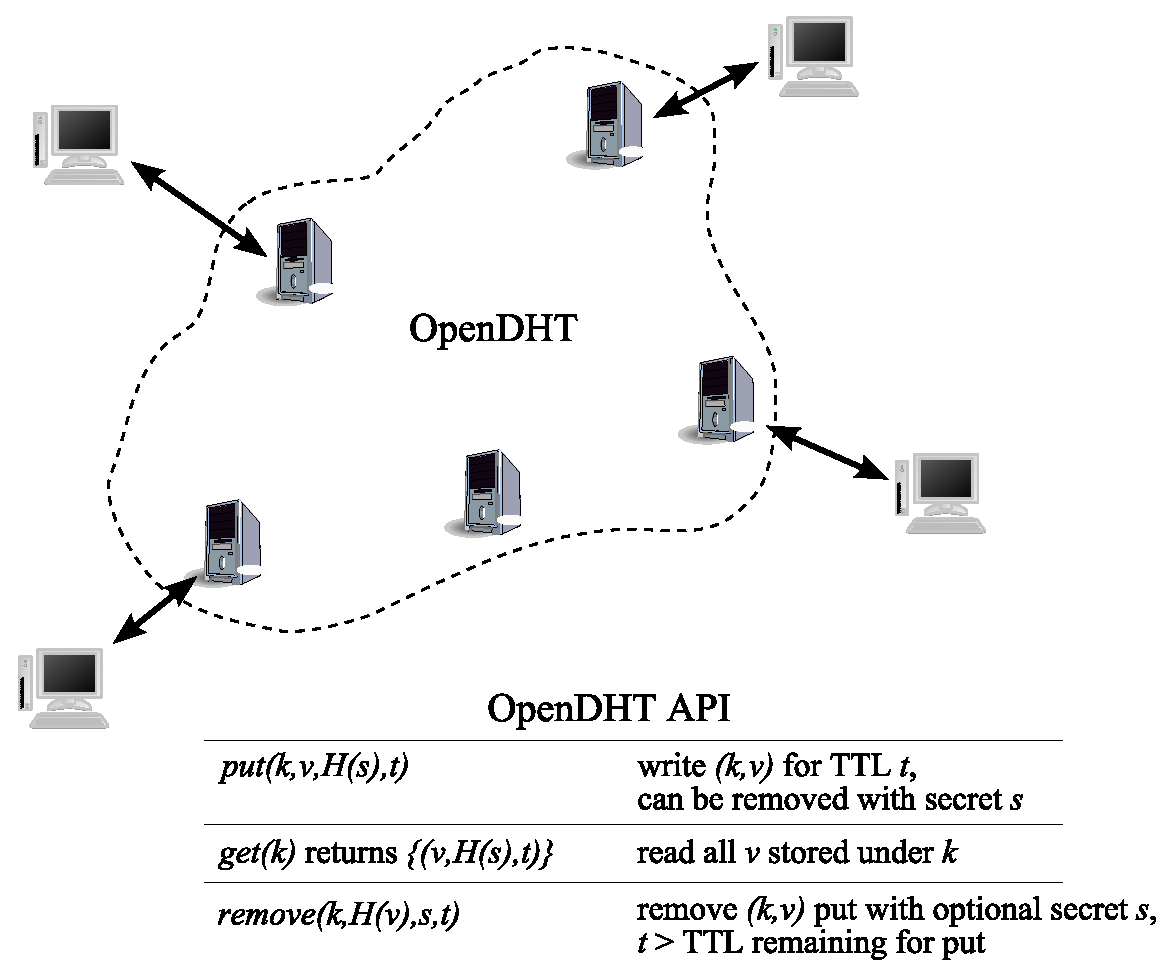
\includegraphics[width=12cm]{pics/opendht.eps}
  \caption{OpenDHT Description.}
  \label{fig:opendht_description}
\end{figure}
\subsection{Workload}
In most experiments we will choose a single file or a set of small files to download, then will vary the rate of clients requesting the file.

\subsection{Metrics}
We will run experiments and log all events and messages, then process logs to calculate the appropriate metrics.  Specific measurements will be client download and upload rates and times, server upload rates, total throughput of the system, total bytes uploaded by clients, and total bytes uploaded by the server.  For all experiments we will examine the distribution of these metrics across the peers, using averages and percentiles to analyze overall behavior of the system.

\subsection{Experiments}
First we will do a proof-of-concept experiment to see if this system effectively meets the premise of the thesis: automatically switching to peer-to-peer content delivery results in improved download time.  We will use a 100KB file and hold other variables constant (with hard-coded, reasonable values), then exert an increasing client load on a server, up to the rate of saturation for the system.  We will compare this with the same load on a traditional client-server system.   We will use Ruby for the implementation to speed development.  We will consider ourselves successful if we are able to gain two times the speed of the traditional server. %to implement it, as, though slower than compiled languages, it is fast enough to keep up with the network stack.

\subsubsection{Automatic Transition}
After proving that the system is viable, we will then run tests to vary parameters and see the effect this has on the protocol.  We will thereby determine the 'best' values for $T$ (the time before switching to peer to peer content delivery), $R$ (the rate at which we will spontaneously decide to give up on the origin server because it is too slow), and $W$ (the time slot of recency in which to calculate $R$).  These basic experiments will determine settings for parameters that will be used for the rest of the experiments.  We will use a fixed file size of 100KB, and a fixed client arrival rate.  We will fix $b$, the number of neighboring peers from whom to download, at a max of 20, which is shown to be reasonably good \cite{bharambe}).  Block size will always be fixed at 32KB, which is shown to be reasonably effective in \cite{zappala}.  Lingering time will be set at 0s (no lingering).  These experiments will be run for 30 minutes, or until 1000 downloads complete, whichever comes first.  We will use an Apache server to distribute the original files.  We will begin by holding all other variables constant and varying $T$ from .5s to 5s.  Similarly, we will hold all variables constant and vary $R$ from 50Kbps to 1 MBps, and  vary $W$ from 1s to 10s (possibly using an estimated mean weighted average EMWA for download speeds). 

We will next test the system with varying server bandwidths to ensure these values are appropriate for a variety of loads.  We will use the original experiments and vary server bandwidths of 32Kbps, 256KBps, 1Mbps and 2Mbps. 
\subsubsection{Entire Web Site}
We will next examine the ability of our system to serve an entire web site.  We will examine effectiveness with a typical web sized files by using a copy of the BYU home page and its associated objects to examine performance downloading an entire web site.  Block size might make a big difference for small files.  We will experiment with different block sizes to determine the impact of this.  The supposition is that too small of a block size will be detrimental, as will too large.

\subsubsection{Optimizations}
Next we will test the effect of lingering times on system performance.  These tests will be with a fixed file size of 100KB, server bandwidth of 256Kbps, and a request rate of 20/min (10x bandwidth).  We will perform the original experiments and vary lingering time from 0s to unlimited. We expect lingering time on the order of a minute or two will give most of the useful benefit to the system. % ALREADY DONE?

After these we will examine whether optimizations seem necessary, from the above experiments.  If needed, we will repeat these experiments with these features turned on and examine whether they provide a performance improvements.  If necessary, we will experiment with imposing a load control of 3 peers per block accessing the origin server (shown in \cite{slurpie} to be efficient), and avoid the slow last block problem.

Finally, we will compare the performance of our protocol with BitTorrent \cite{coral}. We will repeat the basic experiment with BitTorrent and compare it with our own.

\section {Proposed Thesis Schedule}

Proposal: Nov 12 or so

Basic implementation: Dec 31

First experiments completed Feb 1

Optimizations completed March 1

First draft March 15

Final draft April 1

\section {Contribution to Computer Science}
The major contributions of this thesis will be that it creates what we believe to be a unique client-side system of cooperative web clients that automatically transitions from client server to peer-to-peer delivery as needed.  It is transparent to both the server and the user and is non-intrusive in that users do not download files they do not want.  It will  be appropriate for smaller files and will not require a special purpose DHT.  This contribution could dramatically increase the utility of swarming for everyday web browsing.  This thesis could serve as a useful landmark for examining the scenarios when this tool is helpful, and provide hints for best-practices should it be developed by industry.
%The reason this protocol could be useful to the general populace is that the normal, traditional connection to the origin server may be retained, so normal download may still continue, with the peer-to-peer aspect only increasing the download speed.  It could almost guarantee speed increase, only.  It also has the capacity to significantly speed downloads (almost like the golden bullet of Internet computing).  Imagine, for instance, downloading a file from a poorly provisioned server versus from a peer on the same local network.  Orders of magnitude improvement are possible.  It also has the potential to avoid the dreaded TCP timeout of internet browsing, and make browsing more reliable.  In the experience of the author, downloading using swarming tends to be faster than traditional download from even well-provisioned servers, so this could indeed be useful for the Internet populace.  

Another interesting feature of the system is that it has the potential to be a kind of `backup' for servers, if peers in the system have downloaded files.  Since we only lookup files by their URL, it is possible to download files for servers that have crashed or deleted the original files.  This therefore provides redundancy and reliability for servers that go off-line (see Resurrect \cite{resurrect}) (OpenDHT keeps entries for up to a week).  

There has been some concern about the legality of peer-to-peer protocols in the past.  This algorithm, however, represents a generic peer-to-peer protocol, which will tend to be used with normal web downloads, which tend to be legal, so represents a way of using peer-to-peer downloads for a typically legal end.  File sharing and downloading of movies have given p2p a bad name, so this represents a break from that trend, though could still be used for illegal content.
% put in real thesis \footnote{One benefit of this architecture is it disallows for purely illegal one time downloads, in that there are no 'intermediate' nodes that will go and get the content, from the origin server, in your behalf (like mediators)--therefore you, the peer, must get the first copy, therefore you have to get it.  It releases the protocol from illegal culpability.  The protocol itself--not the users.  It also doesn't need a centralized infrastructure.

It therefore provides an automatic transition, and also will help us understand how to combine a larger system (BitTorrent style swarming) with a system suitable for small files.

\section {Delimitations of Thesis}
We do not plan on running tests in a mix of normal peers and `swarming-enabled' peers, which would be indicative of a real world trial.  We are also not looking at the possibility of a server redirecting "non-aware" clients to peers that would be willing to serve it to them (similar to pseudo-servers \cite{pseudoserving}).  Nor do we plan on using traces of real world traffic, as the tests listed should be descriptive enough of the protocol.

We also plan on running experiments mostly on clients that tend to have high upload links--which is not truly indicative of a real-world experience (where most links are assymetric).

A means of verifying that content is not corrupted or maliciously modified is also lacking.  A server that is aware of the protocol could potentially sign checksums and place them in the DHT, or, alternatively, clients could form a reputation system, such as 'voting' on the contents of a block.  Analysis of this is not included in this work.
%\footnote{In the Dijjer system, if a block is found to corrupt this fact is disseminated 'flood-like' through the system.}.  EXPLAIN Dijjer in final thesis

